%%%%%%%%%%%%%%%%%%%%%%%%%%%%%%%%%%%%%%%%%
% baposter Landscape Poster
% LaTeX Template
% Version 1.0 (11/06/13)
%
% baposter Class Created by:
% Brian Amberg (baposter@brian-amberg.de)
%
% This template has been downloaded from:
% http://www.LaTeXTemplates.com
%
% License:
% CC BY-NC-SA 3.0 (http://creativecommons.org/licenses/by-nc-sa/3.0/)
%
%%%%%%%%%%%%%%%%%%%%%%%%%%%%%%%%%%%%%%%%%

%----------------------------------------------------------------------------------------
%	PACKAGES AND OTHER DOCUMENT CONFIGURATIONS
%----------------------------------------------------------------------------------------

\documentclass[landscape,a0paper,fontscale=0.285]{baposter} % Adjust the font scale/size here

\usepackage{graphicx} % Required for including images
\graphicspath{{figures/}} % Directory in which figures are stored

\usepackage{wrapfig}

\usepackage{graphicx}
\usepackage{caption}
\usepackage{subcaption}
\usepackage{epstopdf}

\usepackage{amsmath} % For typesetting math
\usepackage{amssymb} % Adds new symbols to be used in math mode
\DeclareMathOperator*{\argmin}{arg\,min}
\newcommand{\Prob}{\textit{Pr}\ \!}
\newcommand{\vect}[1]{\mathbf{#1}}

\usepackage{booktabs} % Top and bottom rules for tables
\usepackage{enumitem} % Used to reduce itemize/enumerate spacing
\usepackage{palatino} % Use the Palatino font
\usepackage[font=small,labelfont=bf]{caption} % Required for specifying captions to tables and figures

\usepackage{multicol} % Required for multiple columns
\setlength{\columnsep}{1.2em} % Slightly increase the space between columns
\setlength{\columnseprule}{0mm} % No horizontal rule between columns

\usepackage{tikz} % Required for flow chart
\usetikzlibrary{shapes,arrows} % Tikz libraries required for the flow chart in the template

\newcommand{\compresslist}{ % Define a command to reduce spacing within itemize/enumerate environments, this is used right after \begin{itemize} or \begin{enumerate}
\setlength{\itemsep}{1pt}
\setlength{\parskip}{0pt}
\setlength{\parsep}{0pt}
}

\definecolor{lightblue}{rgb}{0.145,0.6666,1} % Defines the color used for content box headers

\begin{document}

\begin{poster}
{
columns=3,
headerborder=closed, % Adds a border around the header of content boxes
colspacing=1em, % Column spacing
bgColorOne=white, % Background color for the gradient on the left side of the poster
bgColorTwo=white, % Background color for the gradient on the right side of the poster
borderColor=lightblue, % Border color
headerColorOne=black, % Background color for the header in the content boxes (left side)
headerColorTwo=lightblue, % Background color for the header in the content boxes (right side)
headerFontColor=white, % Text color for the header text in the content boxes
boxColorOne=white, % Background color of the content boxes
textborder=roundedleft, % Format of the border around content boxes, can be: none, bars, coils, triangles, rectangle, rounded, roundedsmall, roundedright or faded
eyecatcher=true, % Set to false for ignoring the left logo in the title and move the title left
headerheight=0.1\textheight, % Height of the header
headershape=roundedright, % Specify the rounded corner in the content box headers, can be: rectangle, small-rounded, roundedright, roundedleft or rounded
headerfont=\Large\bf\textsc, % Large, bold and sans serif font in the headers of content boxes
%textfont={\setlength{\parindent}{1.5em}}, % Uncomment for paragraph indentation
linewidth=2pt % Width of the border lines around content boxes
}
%----------------------------------------------------------------------------------------
%	TITLE SECTION 
%----------------------------------------------------------------------------------------
%
{
\includegraphics[height=6em]{cde_tag_black.png}} % First university/lab logo on the left
{\bf\textsc{Doctor of Engineering (EngD) in Digital Entertainment, 1st year}\vspace{0.5em}} % Poster title
{\textsc{ Garoe Dorta Perez, Ieva Kazlauskaite and Richard Shaw  \hspace{12pt} University of Bath}} % Author names and institution
{
\includegraphics[height=5em]{Bathlogo.jpg}} % Second university/lab logo on the right

%----------------------------------------------------------------------------------------
%	INVERSE KINEMATICS
%----------------------------------------------------------------------------------------

\headerbox{Inverse Kinematics}{name=objectives,column=0,row=0}{

\begin{center}
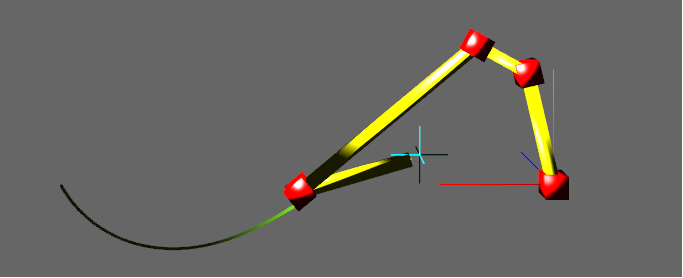
\includegraphics[width=0.8\linewidth]{chain3Dexamplev2}
\end{center}

Inverse kinematics uses a known end-effector position $\mathbf{E}$ to calculate the required angles $\boldsymbol\theta$ between the parts which ensure that the object reaches the desired target position, such that 
\begin{equation*}
\begin{aligned}
\mathbf{E} &= f(\boldsymbol\theta) \rightarrow \boldsymbol{\theta} = f^{-1}(\mathbf{E}) \\  \partial \mathbf{E} &\approx J(\boldsymbol\theta) \partial \boldsymbol\theta \rightarrow \partial \boldsymbol{\theta} \approx J^{-1}(\partial\mathbf{E}),
\end{aligned}
\end{equation*}
where $f$ is the forward kinematics solver, $J$ is the Jacobian matrix, and $J^+ = (J^T J)^{-1}J^T$ is the pseudoinverse of $J$.

% \vspace{0.3em} % When there are two boxes, some whitespace may need to be added if the one on the right has more content
}

%----------------------------------------------------------------------------------------
%	FONT REGRESSION
%----------------------------------------------------------------------------------------

\headerbox{Gaussian Processes}{name=introduction,column=1,row=0,span=1}{
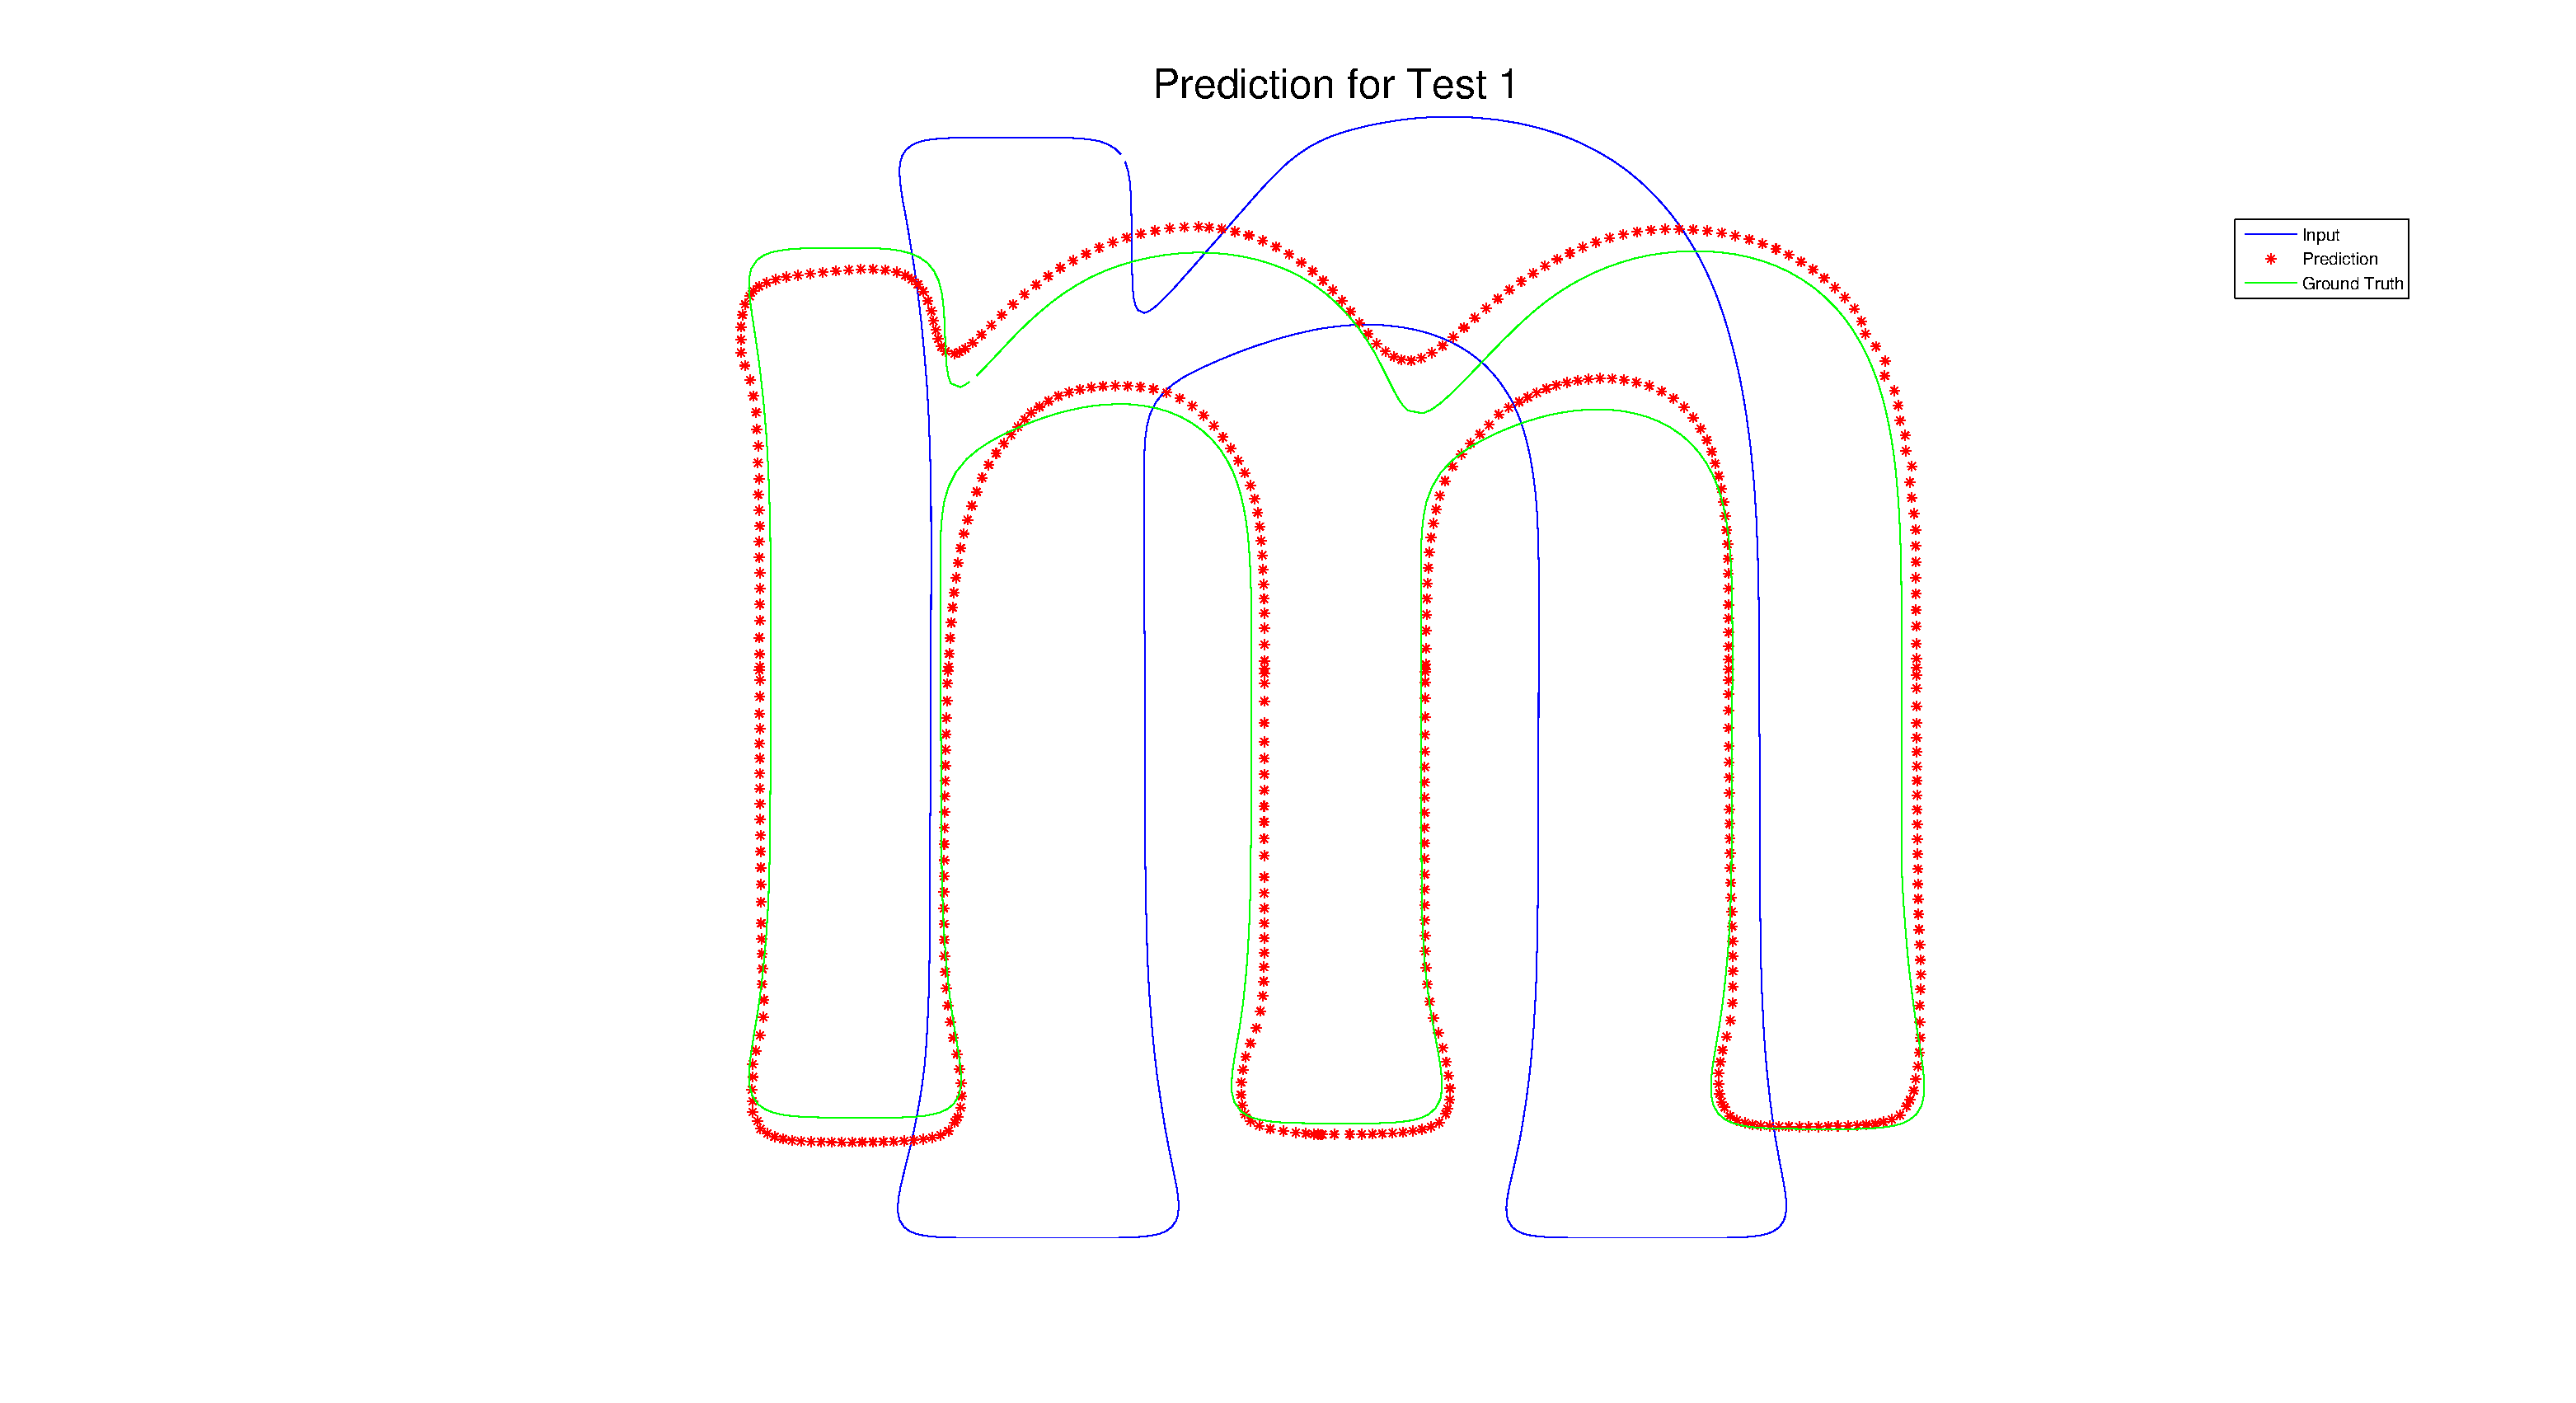
\includegraphics[trim = 120mm 20mm 120mm 20mm, clip, width=0.27\linewidth]{font1}
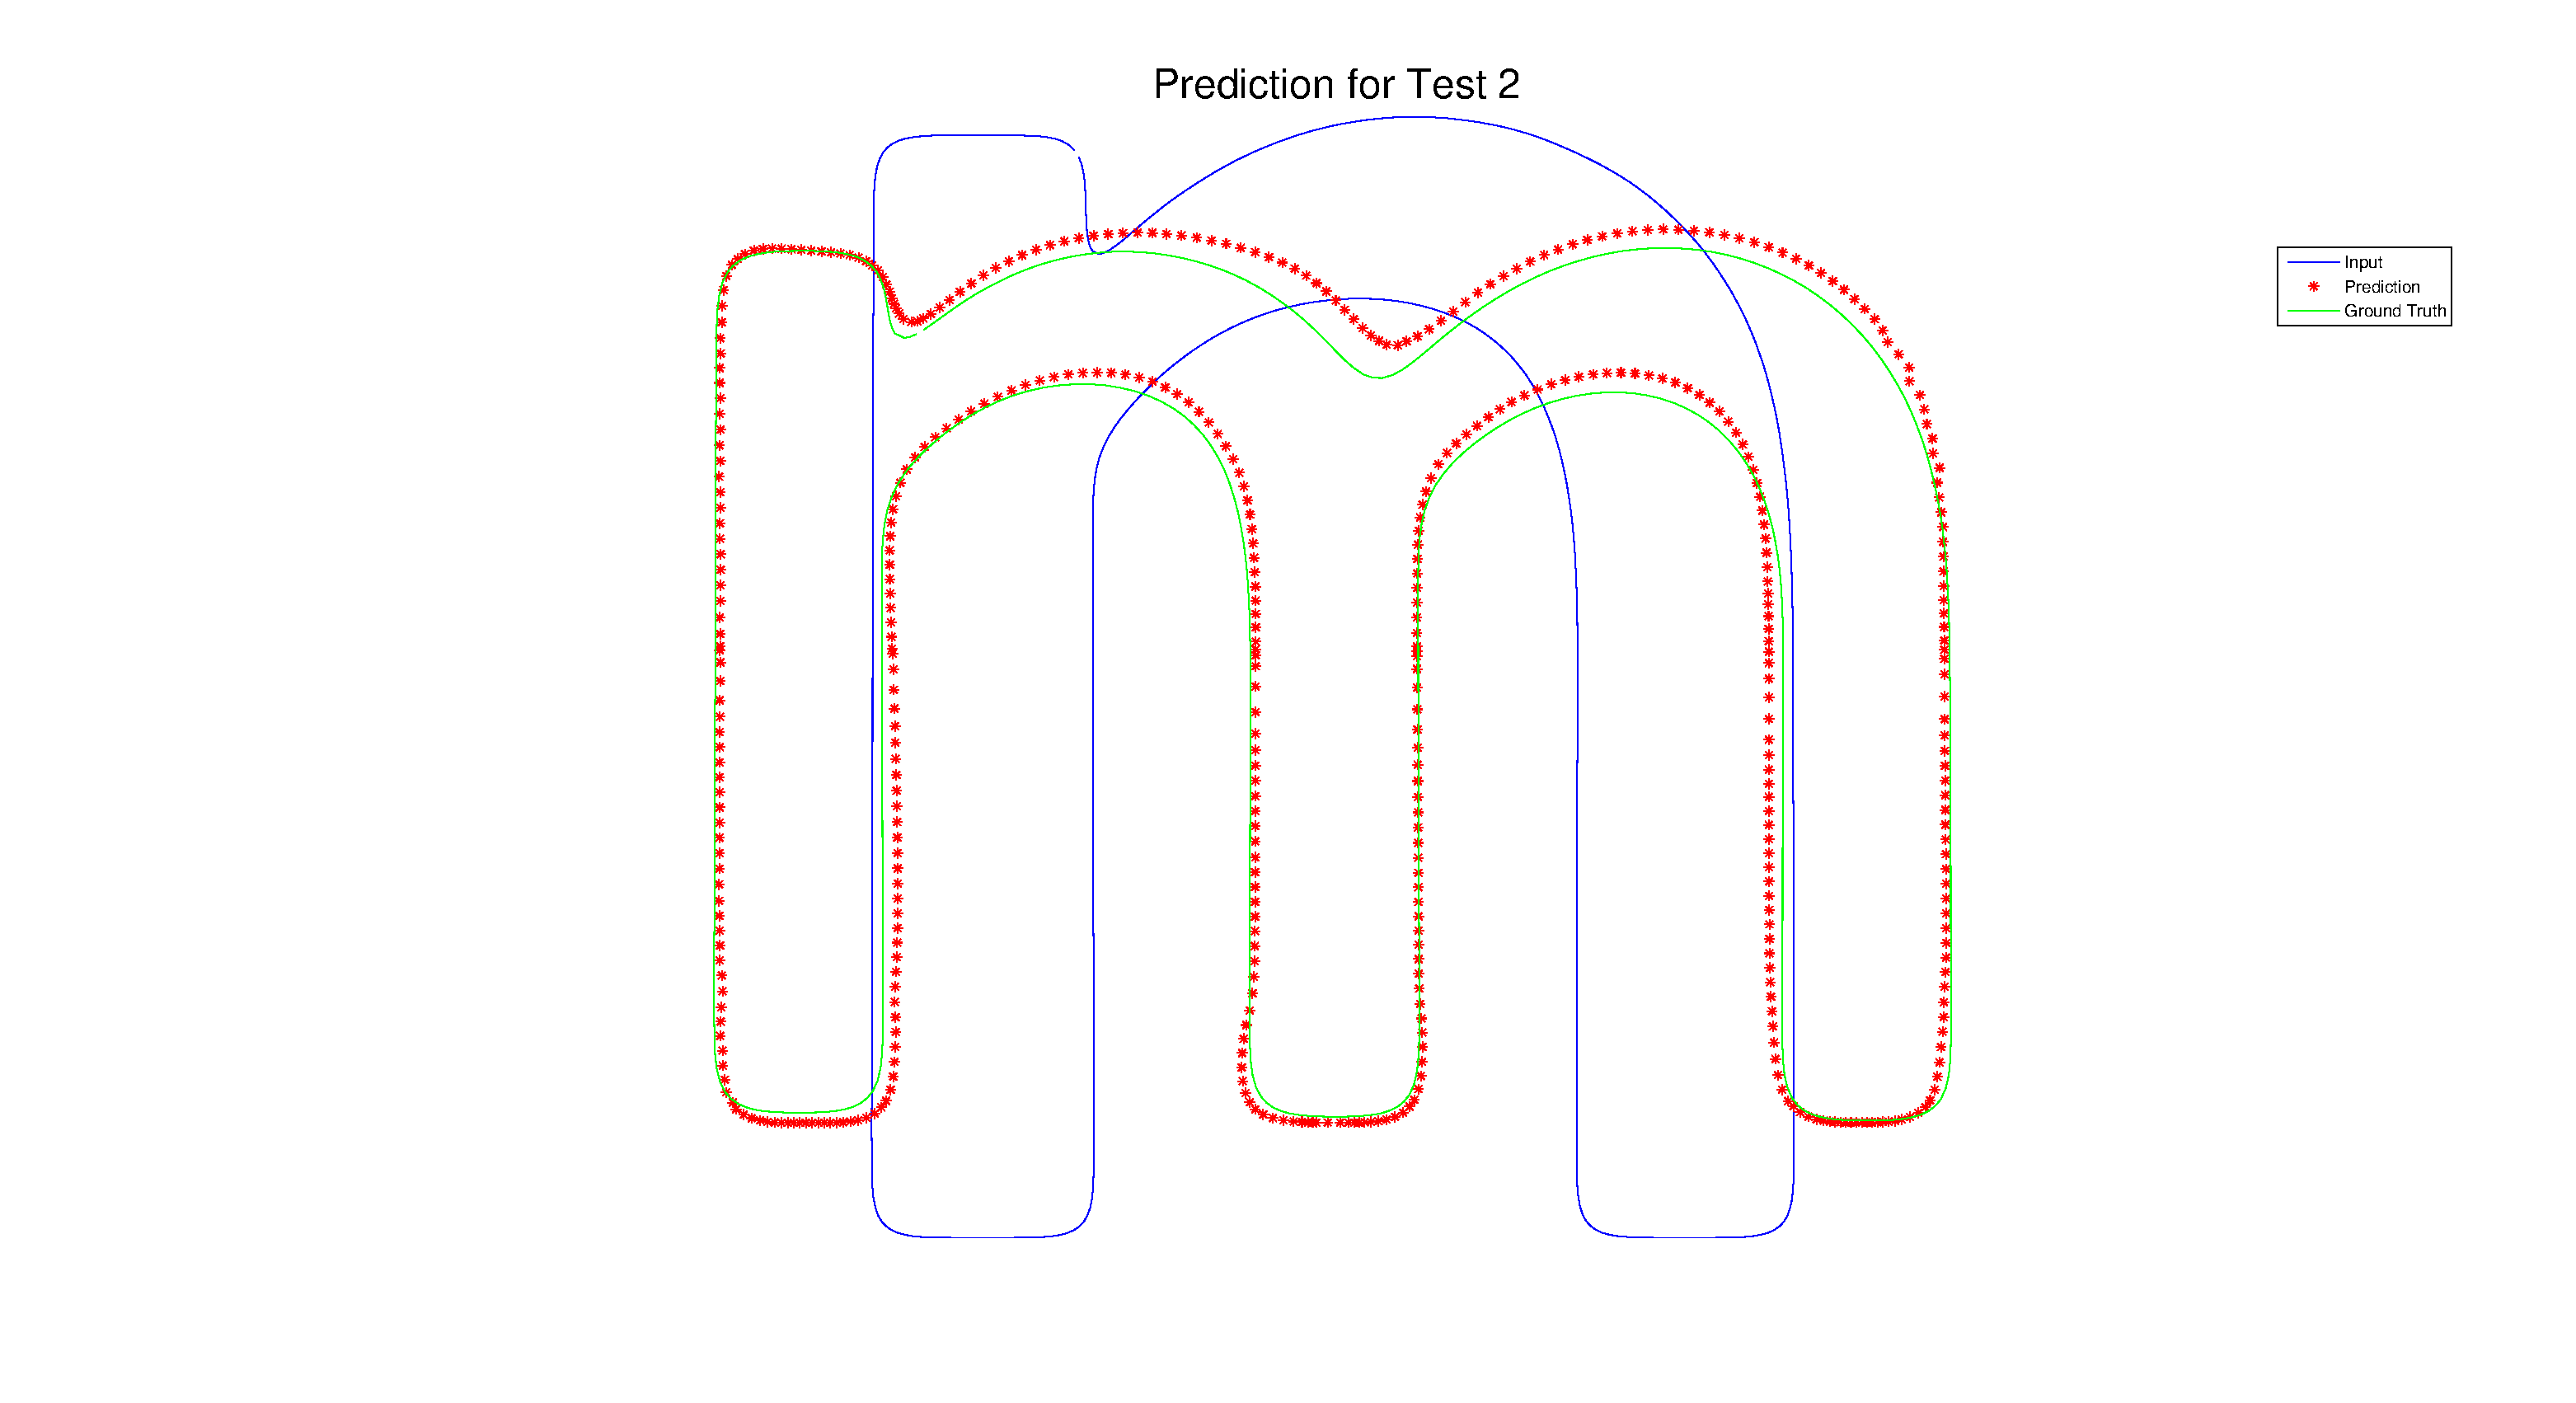
\includegraphics[trim = 120mm 20mm 120mm 20mm, clip,width=0.27\linewidth]{font2}
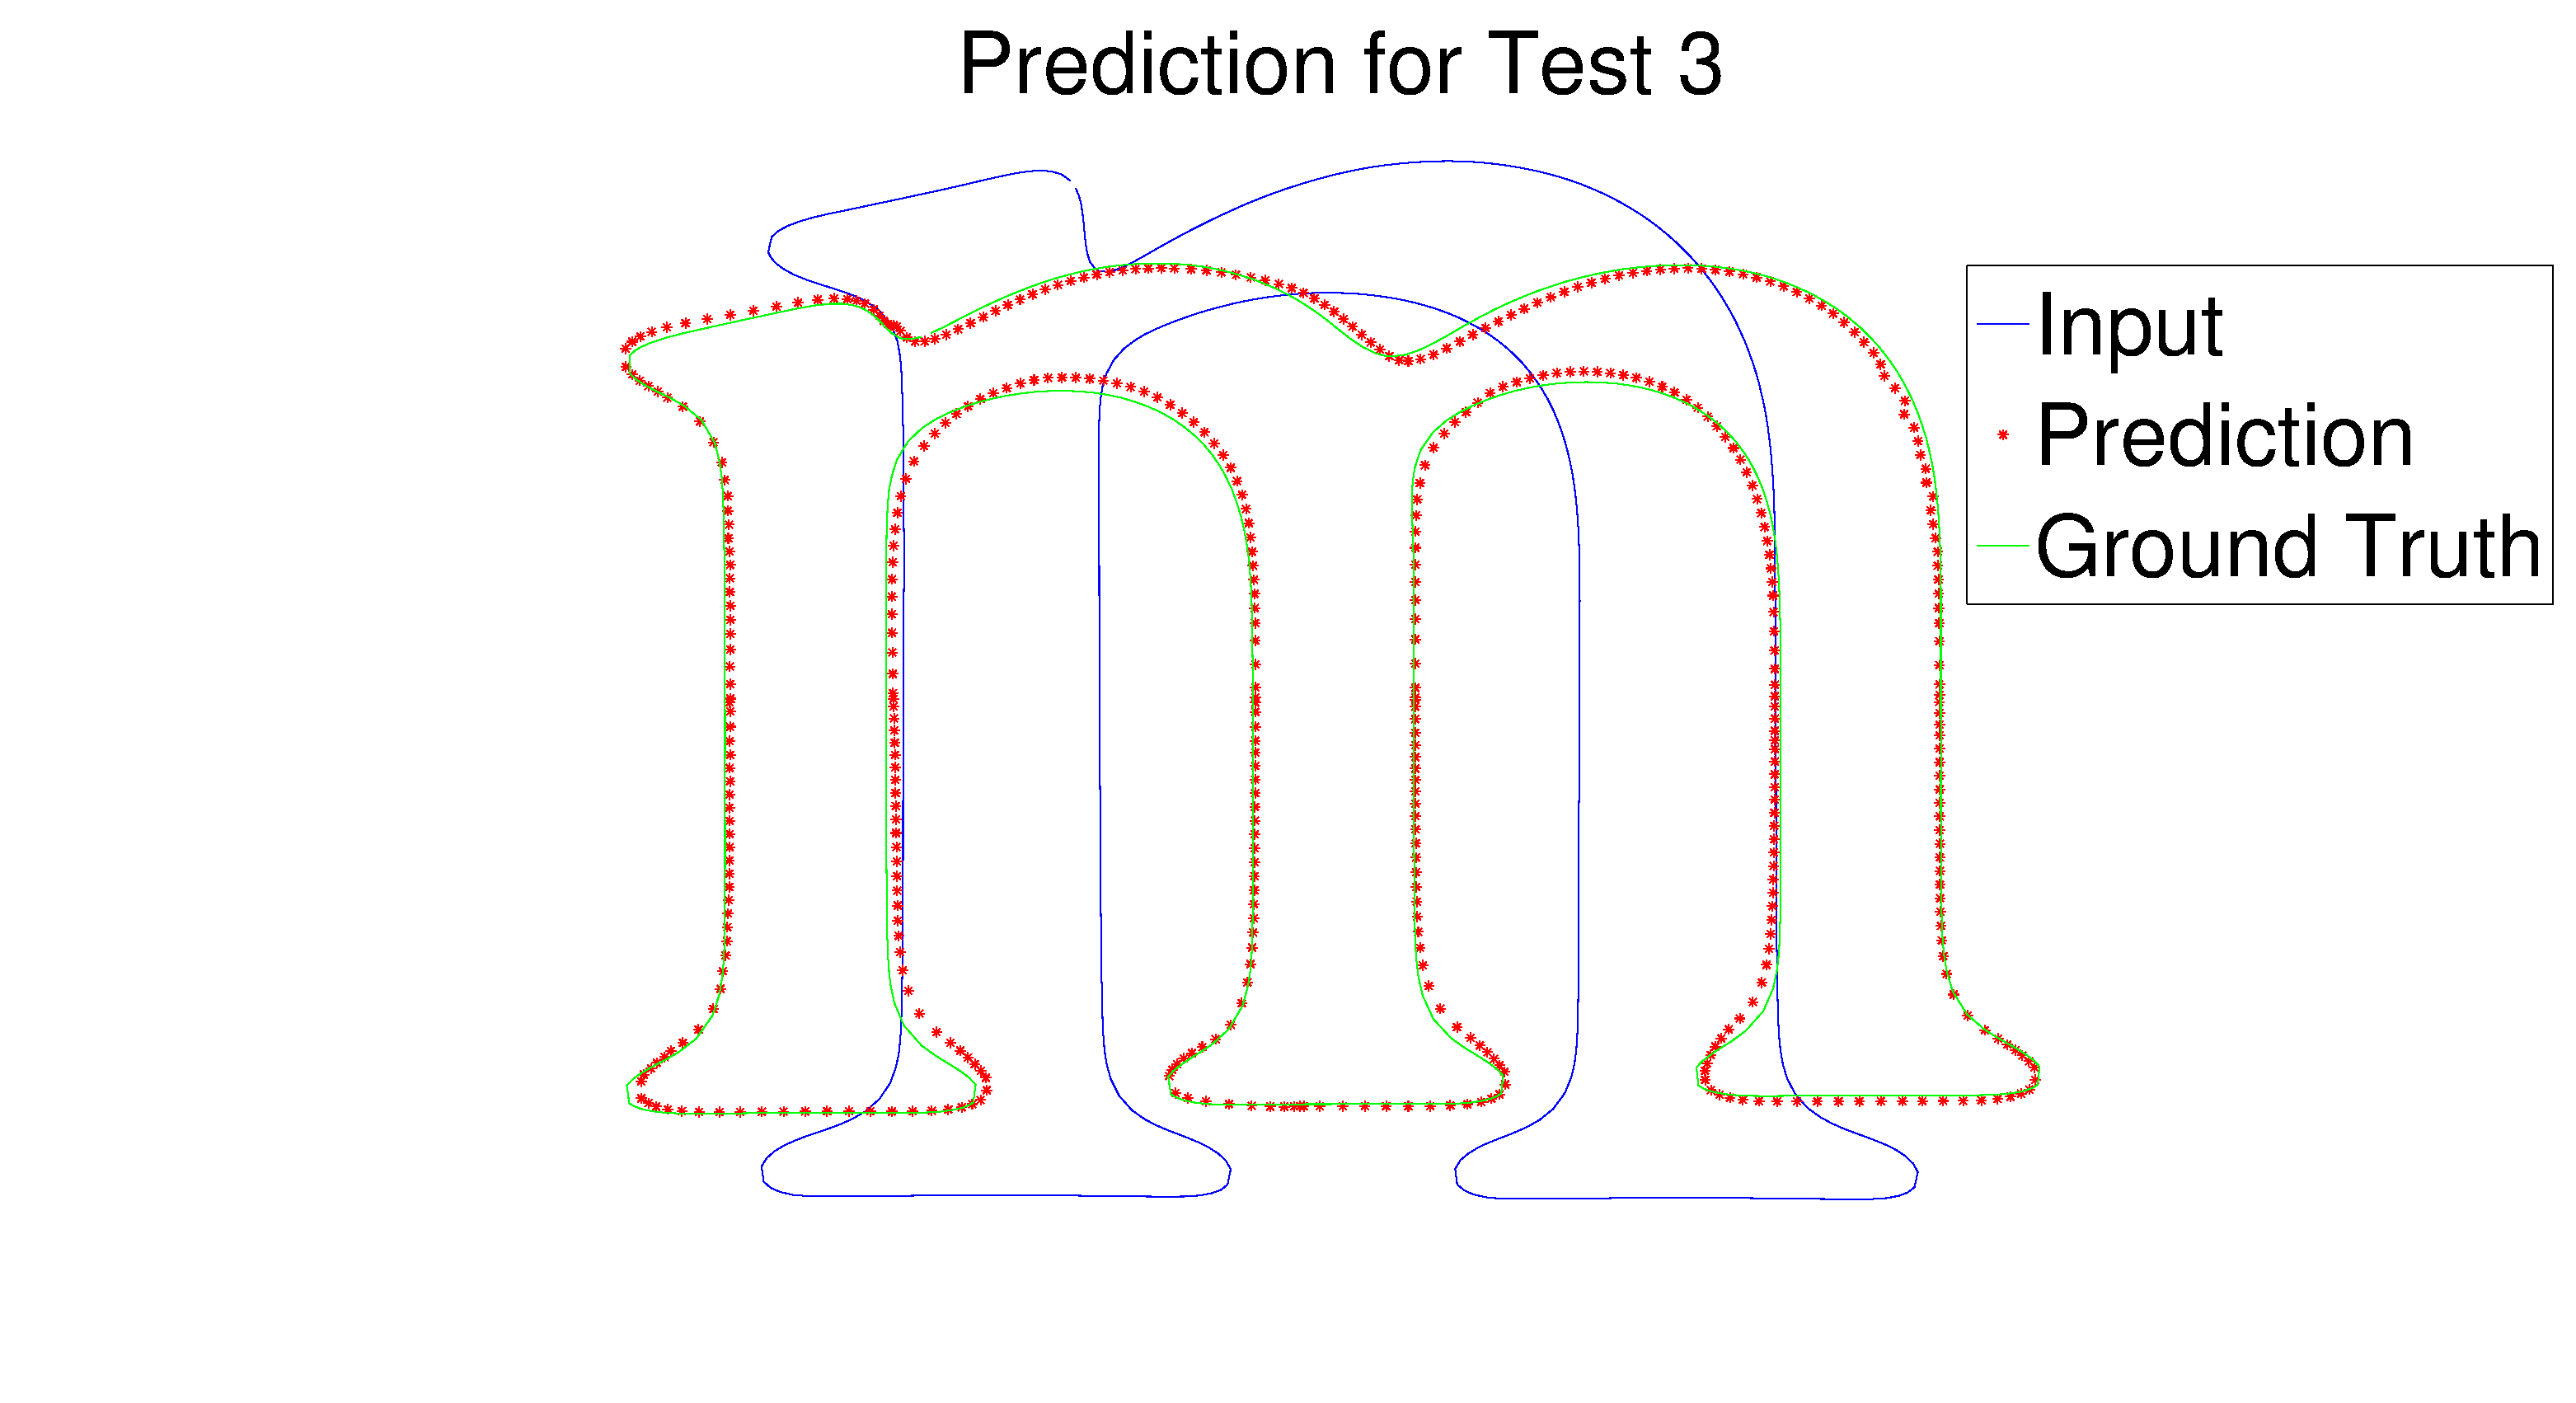
\includegraphics[trim = 120mm 20mm 0mm 20mm, clip,width=0.4\linewidth]{font3}

A Gaussian process is a random process that can be considered as an infinite-dimensional generalisation of the multivariate Gaussian distribution. The main assumption of Gaussian process regression is that our data can be represented as a sample from a multivariate normal distribution. A kernel function $k(x,x')$ must be chosen, and its parameters tuned to maximise the marginal likelihood $\Prob (\boldsymbol{\theta}|\vect{X,w})$
\vspace{0.5pt}
\begin{equation*}
k(x,x') = \sigma_f^2 \exp \left[ {-(x-x')^2} \backslash {2\lambda^2}  \right]
\end{equation*}

Gaussian processes were used to predict the shape of fonts, given a training set. Even with very few training examples, the Gaussian process model gives a reasonable prediction of the shape of a font. The best results were achieved using an exponential kernel with optimised length scale and variance hyperparameters. %
}

%----------------------------------------------------------------------------------------
%	SIFT
%----------------------------------------------------------------------------------------

%\headerbox{SIFT Features}{name=results,column=2,span=1,row=0}{

%}

%----------------------------------------------------------------------------------------
%	REFERENCES
%----------------------------------------------------------------------------------------

\headerbox{References}{name=references,column=0,above=bottom}{

\renewcommand{\section}[2]{\vskip 0.03em} % Get rid of the default "References" section title
\nocite{*} % Insert publications even if they are not cited in the poster
\small{ % Reduce the font size in this block
\bibliographystyle{unsrt}
\bibliography{cde_poster} % Use sample.bib as the bibliography file

}}

%----------------------------------------------------------------------------------------
%	FUTURE RESEARCH
%----------------------------------------------------------------------------------------

\headerbox{Future Research}{name=futureresearch,column=1,span=1,above=bottom}{ % This block is as tall as the references block
The students undertake an individual three-month summer project in a chosen research area before starting the industrial placement.
}

%----------------------------------------------------------------------------------------
%	CONTACT INFORMATION
%----------------------------------------------------------------------------------------

\headerbox{Contact Information}{name=contact,column=2,above=bottom}{ % This block is as tall as the references block

\begin{description}\compresslist
\item[Web] http://www.digital-entertainment.org
\item[Garoe Dorta Perez] g.dorta.perez@bath.ac.uk 
\item[Ieva Kazlauskaite] ik359@bath.ac.uk 
\item[Richard Shaw] richard.o.shaw@gmail.com
\end{description}
}


%----------------------------------------------------------------------------------------
%	PERFORMANCE-DRIVEN FACIAL ANIMATION
%----------------------------------------------------------------------------------------

\headerbox{Performance-driven Facial Animation}{name=conclusion,column=2,span=1,row=0,above=contact}{

\begin{center}
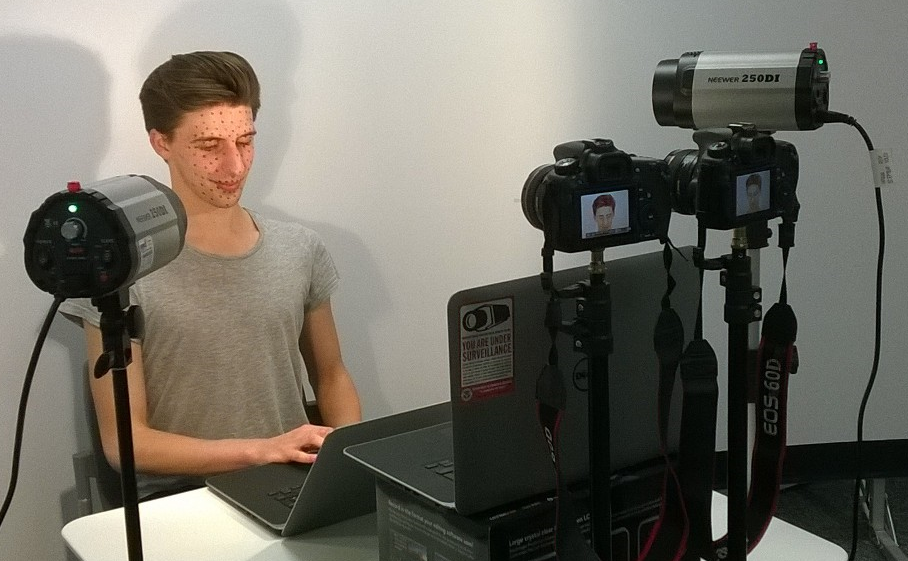
\includegraphics[height=3.0cm]{facecapture}
\end{center}

\begin{center}
\includegraphics[width=1.0\linewidth]{faceprocess_jpg}
\end{center}

A facial performance is captured using calibrated stereo cameras and tracking markers on the face. The marker positions produce a sparse 3D point cloud, which is in turn used to drive a high-resolution mesh. A new face $\mathbf{x^*}$ can be computed from the `neutral-face' plus a weighted combination of blend-shape faces 
$\{ \mathbf{x}_i \}^N_{i=1}$, where the required weights $\vect{w} = \{w_1...w_N\}$ are found through an optimisation procedure
\vspace{-10pt}
\begin{equation*}
\mathbf{x^*} = \sum^N_{i=1} w_i \mathbf{x}_i \quad
\mathbf{w} =
\argmin_{\mathbf{w}} || \mathbf{x^*} - \sum^N_{i=1} w_i \mathbf{x}_i ||^2
\end{equation*}

The synchronised cameras are pre-calibrated using a checkerboard pattern and the intrinsic matrix $\mathbf{K}$ and external parameters $\mathbf{R}$ and $\mathbf{t}$ are recovered from the projection matrices $\mathbf{P}$ and $\mathbf{P'}$, where
\vspace{-5pt}
\begin{equation*}
	\mathbf{u} = \mathbf{PX} = 
  \vect{K}[\vect{R}|\vect{t}]
    \mathbf{X} 		 
\end{equation*}

The fundamental matrix $\mathbf{F}$ encompasses the intrinsic geometry between the two views and defines the epipolar constraint
$\vect{u'}^T \vect{Fu} = 0$
from which we compute epipolar lines and rectify the stereo images to make the correspondence problem easier. Tracked facial points are constrained to lie on epipolar lines so that they intersect at points in 3D space. The captured sparse performance is then mapped to the detailed face mesh using the thin plate splines algorithm. 

}

%----------------------------------------------------------------------------------------
%	SHAPE INTERPOLATION
%----------------------------------------------------------------------------------------

\headerbox{Shape Interpolation}{name=shapeinterp,column=1,below=introduction,above=futureresearch}{%,bottomaligned=conclusion}{ % This block's bottom aligns with the bottom of the conclusion block
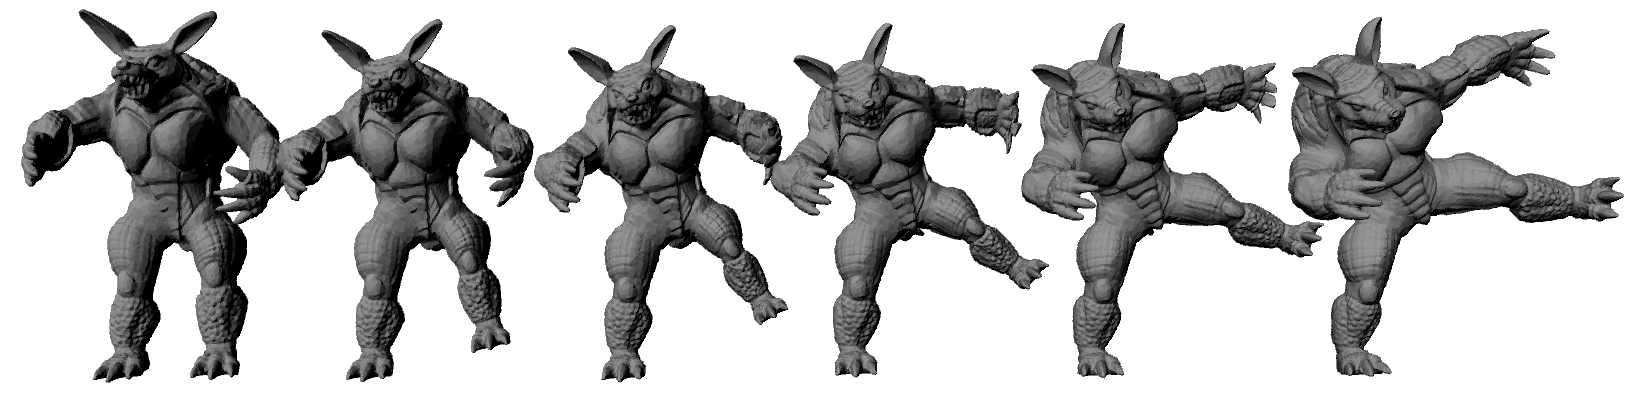
\includegraphics[width=\linewidth]{armadillo_rigid_new} \\
Alexa \textit{et al.} \cite{Alexa:2000} introduced a transformation-based interpolation technique that aims to preserve the structure of the parts that are only translated or rotated between the two meshes. For each triangle, the transformation \(\mathbf{A}\) is split into rotation and translation/shearing, both of which are interpolated linearly. The corresponding smooth transformation is estimated by minimising the error in Frobenius norm:
\vspace{-5pt}
\begin{equation*}
	E_{V(t)} = \sum_{\Delta \in \mathcal{T}} || \mathbf{A}_T(t) - \mathbf{B}_T(t)||^2_F,
\end{equation*} 
where \(V(t)\) are the intermediate positions of vertices, \(\mathbf{A}\) is the ideal mapping, and \(\mathbf{B}\) is the actual affine transformation.

}

%----------------------------------------------------------------------------------------
%	Skin rendering
%----------------------------------------------------------------------------------------
%,bottomaligned=references
\headerbox{Skin Rendering}{name=skinRendering,column=0,below=objectives,above=references}{ % This block's bottom aligns with the bottom of the conclusion block
\begin{center}
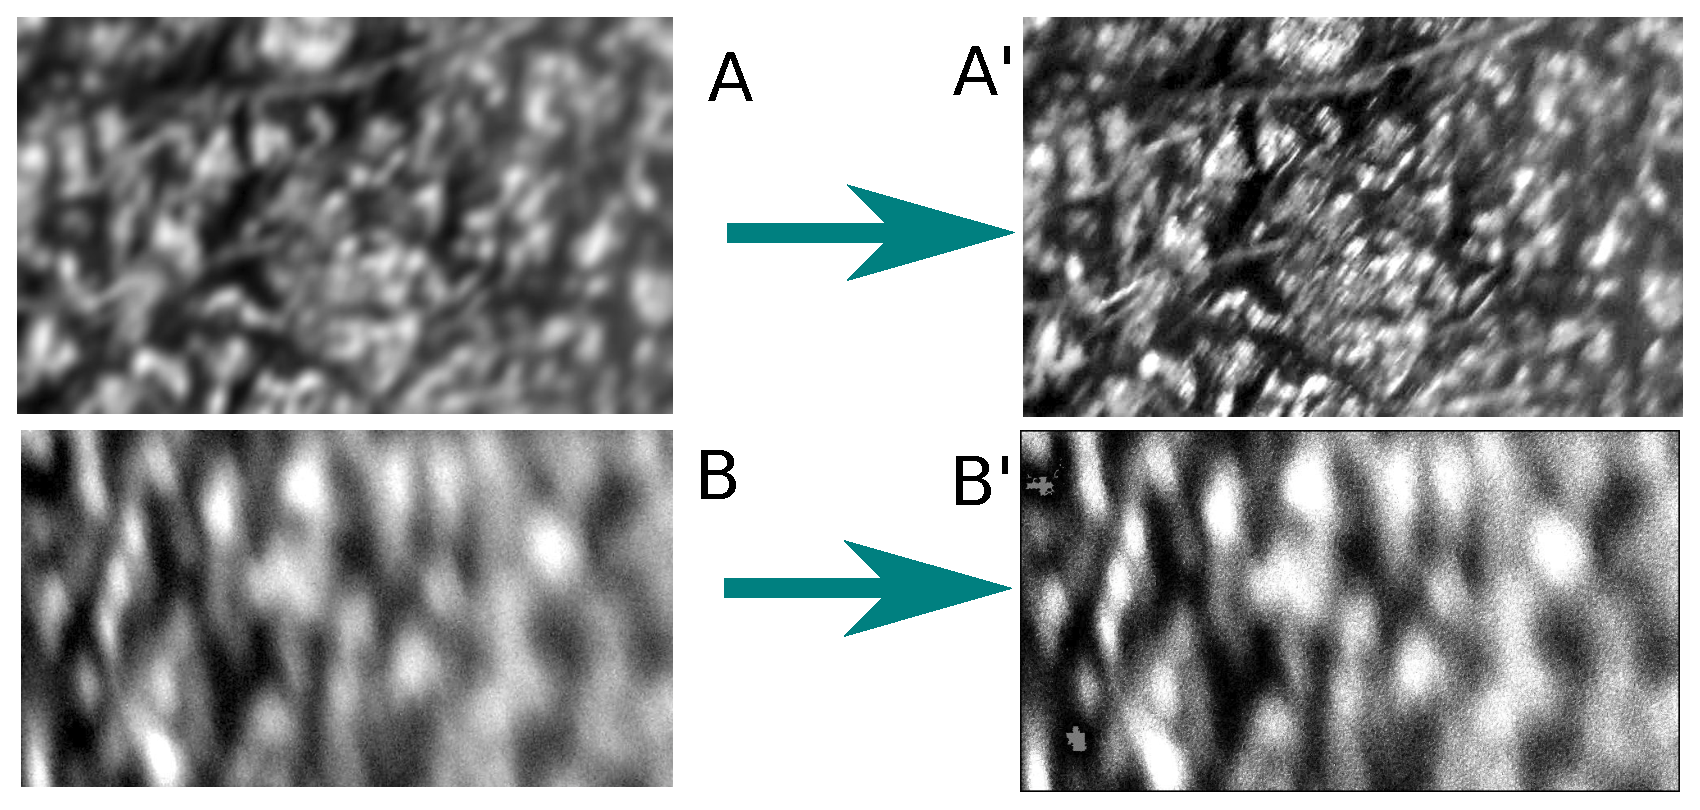
\includegraphics[width=0.9\linewidth]{posterImg}
\end{center}

	Hertzmann \textit{et al.} \cite{Hertzmann:2001} introduced a method to apply filters to images based on a best approximate match and a best coherence match pixel search.
	A high-resolution bump map $B'$ can be synthesised from a lower resolution $B$ and a pair of training samples $A$ and $A'$.
}

%----------------------------------------------------------------------------------------

\end{poster}

\end{document}